\documentclass[11pt]{article}

\usepackage{amssymb,amsmath,amsthm}
\usepackage{verbatim}
\usepackage{fullpage}
\usepackage{gencor}
\usepackage{mathrsfs}
\usepackage{authblk}
\usepackage{graphicx}
\usepackage{caption}
\usepackage{subcaption}
\numberwithin{equation}{section}
\usepackage[nottoc,notlof,notlot,numbib]{tocbibind}
\usepackage{xr-hyper}
\externaldocument[supp-]{supp}

\frenchspacing

\title{Estimating Genetic Correlations between Traits from GWAS Summary Statistics}
\author{Brendan Bulik-Sullivan*, Hilary Finucane*, ... , \emph{et. al.}}

\begin{document}
\maketitle

%%%%%%%%%%%%%%%%%%%%%%%%%%%%%%%%%%%%%%%%%%%%%%%%%%%%%%%%%%%%%%%
\begin{abstract}\label{abstract}
%%%%%%%%%%%%%%%%%%%%%%%%%%%%%%%%%%%%%%%%%%%%%%%%%%%%%%%%%%%%%%%

Discovering relationships between phenotypes is a fundamental goal of epidemiology,
with implications for drug development, nosology and treatment.
The interpretation of phenotypic correlations in observational epidemiological studies 
can be confounded by environmental factors,
so genetic correlations between phenotypes may be more easily interpretable.
The largest currently available sources of genotype-phenotype data are genome-wide association studies (GWAS); 
however, existing methods for estimating genetic correlation from GWAS data require
genotype and phenotype data for at least one of the phenotypes, 
which can be difficult or impossible to obtain due to restrictions on data sharing.
For this reason, only a few dozen genetic correlations have been estimated from GWAS data to date.
In this paper, we describe a method based on LD Score regression
which estimates genetic correlations directly from GWAS summary statistics
and is immune to sample overlap. 
In addition, we relax many common assumptions about genetic architecture, 
and demonstrate that our method is not confounded  
when effect size depends on allele frequency or linkage disequilibrium.
Since dozens of sets of summary statistics can be freely downloaded from the internet,
we can report a much larger number of  genetic correlations 
 -- 300 in this paper alone -- than was previously possible.

\end{abstract}

\newpage
\tableofcontents
\listoffigures
\listoftables
\newpage



%%%%%%%%%%%%%%%%%%%%%%%%%%%%%%%%%%%%%%%%%%%%%%%%%%%%%%%%%%%%%%%
\section{Introduction}
\label{Introduction}
%%%%%%%%%%%%%%%%%%%%%%%%%%%%%%%%%%%%%%%%%%%%%%%%%%%%%%%%%%%%%%%

The additive genetic covariance, $\rho_g$ between two phenotypes $y_1$ and $y_2$ is the bivariate analogue of heritability,
and is defined as the covariance (in the population) between the additive genetic components of $y_1$ and $y_2$. 
The normalized version of genetic covariance is genetic correlation,
\begin{equation}
	r_g := \dfrac{\rho_g}{\sqrt{h^2_1h^2_2}},
\end{equation}
which lies in the interval $[-1,1]$, where $h^2_i$ denotes the heritability of trait $i$.
Note that genetic correlation is a stronger condition than pleiotropy. 
To exhibit genetic correlation,
it is not sufficient for two phenotypes to be influenced by the same genetic loci:
the directions of effect of the variants that influence the phenotypes must also be consistently aligned across the genome.

Existing methods for estimating genetic correlation from GWAS genotype data 
(\emph{e.g.,} restricted maximum likelihood (REML) as implemented in the software package GCTA 
\cite{yang2010, yang2011gcta} -- hereafter referred to as GCTA-REML -- or polgyenic risk scores \cite{dudbridge2013power})
require individual genotype data, which are often difficult or impossible to obtain due to restrictions on data sharing. 
Thus, investigations of additive genetic correlations between human traits 
 typically report at most a handful of genetic correlations, 
usually estimated from samples of at most a few tends of thousands of individuals,
and only a few dozen genetic correlations have been estimated using GWAS data to date
\cite{pgccdg2013, vattikuti2012heritability, chen2014estimation}.

We propose a modification of LD Score regression \cite{buliksullivan2014}
that can estimate the genetic correlation between two traits from GWAS summary statistics. 
Precisely, if $z_{1,j}z_{2,j}$ are the $Z$-scores for a SNP $j$ from two GWAS, $\ell_j$, the LD Score of SNP $j$,
and we assume a simple model of genetic architecture where all SNP effect sizes are drawn in uncorrelated fashion 
from distributions with equal means and variances,
\begin{equation}
		\E[z_{1,j}z_{2,j}] = \dfrac{\rho_g\sqrt{N_1N_2}}{M}\ell_j + \dfrac{N_s\rho}{\sqrt{N_1N_2}},
\end{equation}
where $N_1$ and $N_2$ are the sample sizes of each study, $N_s$ is the number of shared samples,
$\rho$ is the overall phenotypic correlation and $\rho_g$ is the genetic covariance. 
This equation is derived in the supplementary note, and a similar relationship holds if one or both of the studies 
is an ascertained study of a binary phenotype. 
The relationship becomes more complicated if effect sizes are not identically distributed, but instead depend on  
minor allele frequency (MAF) or linkage disequilibrium (LD), as discussed in \cite{speed2012improved}; 
however, we can easily accommodate such dependencies with partitioned LD Score regression 
(as described in the results and methods sections of this paper and also \cite{finucane2014partitioning}).

Thus, if we regress the product $z_{1,j}z_{2,j}$ of $Z$-scores from two GWAS against $\ell_j$, the LD Score of SNP $j$, 
the slope times a constant estimates genetic covariance.
Since sample overlap affects the term $z_{1,j}z_{2,j}$ equally for all SNPs, and the quantity $N_s$ appears only 
as the intercept term, the LD Score regression estimator of genetic covariance is not biased by sample overlap. 
Indeed, if $\rho$ is known (\emph{e.g.,} if both studies assay the same phenotype and $\rho=1$), the intercept 
from this regression times a constant can be used as an estimator of the number of shared samples.
We can estimate heritability using LD Score regression (as described in \cite{buliksullivan2014}),
and use these heritability estimates to transform the estimates of genetic covariance into estimates of genetic correlation.

In this paper, we describe a series of simulations that validate these claims. 
We then replicate the genetic correlations reported by the PGC Cross-Disorder Group using GCTA-REML in \cite{pgccdg2013},
using only the summary statistics from \cite{cross2013identification}, 
before reporting 300 (mostly novel) 
genetic correlations between pairs of phenotypes with publicly available GWAS summary data.
We find that phenotypes generally tend to cluster within categories defined by clinical practice and observational epidemiology; 
nonetheless, we do observe some surprising results.
For instance, we estimate genetic correlations close to zero between Alzheimer's and all of the psychiatric traits;
although Alzheimer?s disease is classified as a psychiatric disorder in ICD-10, it appears to be genetically distinctive. 
Instead, Alzheimer's disease clusters (weakly, but significantly) with anthopometric and metabolic traits.

The computational demands of our method are mild, and we provide an open-source software package, \texttt{ldsc},
written in python, which implements the analyses described in this paper and also the analyses from
\cite{buliksullivan2014, finucane2014partitioning} (URLs).


%%%%%%%%%%%%%%%%%%%%%%%%%%%%%%%%%%%%%%%%%%%%%%%%%%%%%%%%%%%%%%%
\section{Results}\label{Results}
%%%%%%%%%%%%%%%%%%%%%%%%%%%%%%%%%%%%%%%%%%%%%%%%%%%%%%%%%%%%%%%

\subsection{Simulations}
In order to check our derivations and verify the robustness of our inference procedure to 
violations of our modeling assumptions, we performed a variety of simulations. 

\subsubsection{Sample Overlap}
To verify the unbiasedness of our estimation procedure in the presence of sample overlap 
(which is derived formally in the Supplementary Note), 
we simulated two GWAS with quantitative phenotypes,
using genotypes from the 4,292 individuals in the Wellcome Trust Case/Control Consortium 1 
(WTCCC1, \cite{international2011genetic}) bipolar disorder cohort for the first GWAS
and genotypes from the 4,482 individuals in the WTCCC1 coronary artery disease cohort for the second GWAS.
These cohorts contain 2,713 overlapping inviduals. 
Additive genetic effect sizes were drawn from a bivariate point-normal distribution 
with 10\% of SNPs causal and true genetic correlation $0.7$.
We then estimated genetic correlation using LD Score regression.
Results from these simulations are summarized in Supplementary Table \ref{supp-sample_overlap_sim},
and confirm that LD Score regression is not confounded by sample overlap.

\subsubsection{Case-Control Ascertainment}
We simulated ascertained GWAS in order to evaluate the performance of 
LD Score regression under case/control ascertainment.
Simulating case/control GWAS under a liability threshold model requires rejection
sampling from a large pool of individuals.
For instance, in order to simulate drawing 1,000 cases 
for a phenotype with prevalence of $1\%$, 
one would need on expectation to sample 100,000 individuals.
This is impractical, so we used simulated genotypes with a simplified LD block LD structure 
($r^2=0$ or $1$) for simulating ascertainment (this is the same simulation scheme used in \cite{buliksullivan2014}).

We simulated standard case/control ascertainment following a liability threshold model, 
and estimated the genetic correlation using LD Score regression. 
Results from these simulations are summarized in supplementary table \ref{supp-qt_cc_sim},
and confirm that LD Score regression recovers the true heritability and genetic correlation, 
even for low-prevalence diseases.
The simplified LD structure should not hinder interpretation of these simulation results, 
especially since we also provide a proof that unlike GCTA-REML \cite{golan2013narrowing},
LD Score regression is valid when applied to ascertained samples of binary phenotypes (Supplementary Note).


%\subsubsection{Complicated Ascertainment}

%%% TODO WRITE ME %%%%

%Next, we simulated a more complicated ascertainment scheme,
%representative of the study design used by many large GWAS consortia,
%where all case samples are independent, 
%but there is a large pool of healthy controls 
%(\emph{i.e.,} individuals who are controls for both phenotypes)
%shared between all studies.
%...
%We caution that while LD Score regression estimates of genetic correlation are robust to
%standard case/control ascertainment and the healthy controls model of ascertainment, 
%it can be difficult to interpret LD Score regression estimates of genetic covariance 
%obtained from GWAS with more complicated ascertainment schemes.
%As an example, 
%if one were to attempt to estimate the genetic correlation between body-mass index (BMI) and type-2 diabetes (T2D)
%using LD Score regression and summary statistics from a non-ascertained GWAS for BMI
%and a GWAS for T2D consisting of high-BMI controls and low-BMI cases,
%then the resulting estimate would not be on a readily-interpretable scale.

\subsubsection{Misspecified Models of Genetic Architecture}

Estimates of heritability and genetic covariance can be biased if the underlying model of genetic architecture is misspecified.
For example, Speed, \emph{et. al.} \cite{speed2012improved} 
demonstrate that GCTA-REML is confounded by MAF- or LD-dependent genetic architectures.
Estimates of genetic correlation are somewhat more robust.
Since genetic correlation is estimated as a ratio $\hat{\rho}_g / \sqrt{\hat{h}^2_1\hat{h}^2_2}$
(or the weighted block jackknife estimator of this ratio, see Methods),
and the model misspecification bias affects both the numerator and the denominator in the same direction,
the bias will tend to approximately cancel, unless genetic correlation 
(not just heritability and genetic covariance) also depends on MAF or LD.
Naive LD Score regression is subject to similar biases as REML; however,
it is possible to remove these biases by allowing for MAF- or LD-dependent genetic architectures by using partitioned LD 
Score regression (see \cite{finucane2014partitioning} and Methods)

We used simulations to explore the behavior of both naive and partitioned LD Score regression 
under various nonstandard models of genetic architecture. 
We simulated three sets of bivariate genetic architectures with MAF- and LD-dependence.

For the first genetic architecture,
the MAF- and LD- dependence was the same for both phenotypes and genetic correlation did not vary with MAF or LD. 
Effect sizes were drawn from a normal distribution so that the magnitude of per-allele effect sizes were uncorrelated with MAF and variants with LD Score below 100 were $4\times$ enriched for heritability.

For the second genetic architecture, 
the genetic correlation did not vary with MAF or LD, 
but the direction of the MAF- and LD-dependence was different for each phenotype
We drew per-allele effect sizes for the first phenotype from a normal distribution 
such that the variance of per-allele effect sizes were uncorrelated with MAF, 
and variants with LD Score below 100 were $4\times$ enriched for heritability.
Per-allele effect sizes for the second phenotype were drawn from a normal distribution 
such that the variance of per-allele effect size followed $\sqrt{p(1-p)}$, 
where $p$ is MAF, and variants with LD Score above 100 were $4\times$ enriched for heritability. 

For the third genetic architecture, we allowed not only heritability and genetic covariance to depend on MAF and LD,
but also genetic correlation. 
The parameters of these simulations were the same as the second genetic architecture, 
except that genetic correlation was 0.2 for variants with LD Score less than 100 and 0.8 for variants with LD Score greater than 100. 

We  estimated heritability, genetic covariance and genetic correlation using both naive LD Score regression 
and two partitioned LD Score regression models (one with 30 bins, one with 60 bins) 
that allow for both MAF- and LD-dependence.
Results from these simulations are presented (in the order described) in Supplementary Tables 
\ref{supp-parallel}, \ref{supp-antiparallel} and \ref{supp-depcor}.
The heritability and genetic covariance estimates from naive LD Score regression are badly biased in all cases
(which is similar to the results obtained by Speed, \emph{et. al.}), 
but the bias in the genetic correlation estimates was much less severe, except in the third set of simulations,
where genetic correlation varied with LD.
However, as expected, partitioned LD Score regression was able to remove almost all bias introduced by 
LD- and MAF-dependence,
and the increase in the standard errors was only mild.



%%%%%%%%%%%%%%%%%%%%%%%%%%%%%%%%%%%%%%%%%%%%%%%%%%%%%%%%%%%%%%%
\subsection{Real Data}\label{Real Data}
%%%%%%%%%%%%%%%%%%%%%%%%%%%%%%%%%%%%%%%%%%%%%%%%%%%%%%%%%%%%%%%

\subsubsection{Replication of PGC Cross Disorder Results}

As a sanity check, we replicated the estimates of genetic correlations between psychiatric phenotypes obtained with
individual genotypes and GCTA-REML in the PGC Cross-Disorder Group paper \cite{pgccdg2013}, 
using LD Score regression and the summary statistics from \cite{cross2013identification},
downloaded from the PGC website (URLs).
For this replication, we used an LD Score with $r^2$'s from the 1000 Genomes Europeans \cite{10002012integrated}
but with the sum of $r^2$'s taken only over the 1.2 million autosomal HapMap 3 SNPs \cite{international2010integrating} 
retained for LD Score regression in \cite{buliksullivan2014}
(hereafter referred to as HapMap3 LD Score).
We did this to match the model of genetic architecture fit by GCTA-REML,
where only the effects of genotyped SNPs are modeled. 
With standard LD Score regression, we can model the effects of SNPs that are not genotyped in the GWAS,
because we have LD information about these SNPs from a sequenced reference panel.
(see the section ``LD Score Regression is Haseman-Elston Regression'' in the Supplementary Note). 
We believe that our partitioned LD Score regression model is more reliable, so we fit the GCTA-REML model
simply as a technical demonstration.
The genetic correlations estimates in the next section (``Application to a Large Set of Publicly Available Summary Statistics")
are more reliable, since they use the partitioned LD Score regression model and much larger sample sizes.

Nonetheless, when we fit the GCTA-REML model using LD Score regression
we replicated the results from the PGC Cross-Disorder Group paper closely, 
and the standard errors were similar to those obtained from GCTA-REML,
except for the smallest studies (Attention Deficit Hyperactivity Disorder, Autism)
(Figure \ref{Fig:Replication of PGC Cross Disorder Results}).
In general, we expect the standard errors from GCTA-REML to be lower than the LD Score regression standard errors
at fixed sample size when the distributional assumptions 
(normally distributed phenotypes, environmental effects independent of genetic effects in the sample) 
made by GCTA-REML are met, which will often be the case for non-ascertained studies of quantitative traits.
In ascertained studies of binary phenotypes, the distributional assumptions made by GCTA-REML do not hold
\cite{golan2013narrowing}, and so it is not surprising that LD Score regression performs about as well in this example.
The computational demands of this analysis were trivial: after computing LD Scores and pre-processing the summary statistics, 
the LD Score regression took about one minute per pair of phenotypes
(most of which was reading compressed LD Score files into memory) 
and less than 1GB of RAM.

\begin{figure}[!ht]

\begin{centering}
\caption{Replication of PGC Cross Disorder Results}
    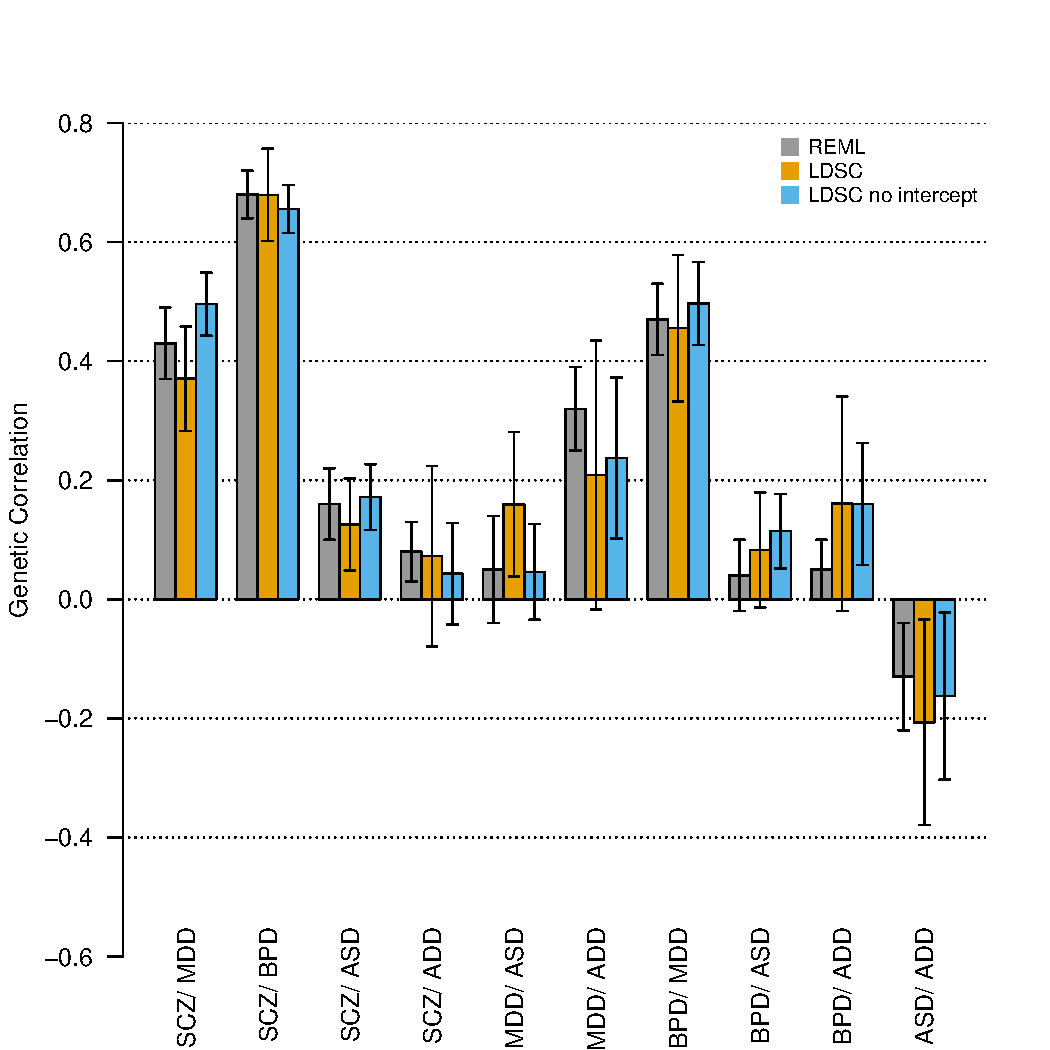
\includegraphics[scale=0.8]{figs/ldsc_vs_gcta.pdf}
         \label{Fig:Replication of PGC Cross Disorder Results}

\end{centering}

This plot compares LD Score regression estimates of genetic correlation using the summary statistics from \cite{cross2013identification} (which were generated from approximately the same data as \cite{pgccdg2013}) 
The horizontal axis indicates pairs of phenotypes, and the vertical axis indicates genetic correlation.
The red bars are the LD Score regression estimates, the blue bars are the GCTA-REML estimates from \cite{pgccdg2013},
and the black lines indicate one standard error (note that it is not clear whether the asymptotic standard errors 
reported by GCTA-REML are valid for small ascertained studies; these may be underestimates). 
For this plot, we used a HapMap3 LD Score (Online Methods), since this more closely corresponds to the model
fit by GCTA-REML (which only models the effects of genotyped SNPs). 
This plot should be interpreted as a technical sanity check. 
The estimates of genetic correlation between psychiatric phenotypes presented under the header 
``Application to a Large Set of Publicly Available Summary Statistics" use larger sample sizes and rely on fewer
assumptions about genetic architecture, and so are more robust.
Abbreviations: 
ADD = Attention Deficit Hyperactivity Disorder (1947 trio cases, 1947 trio pseudocontrols, 840 cases, 688 controls);
ASD = Autism Spectrum Disorder (4788 trio cases, 4788 trio pseudocontrols, 161 cases, 526 controls);
BPD = Bipolar Disorder (6990 cases, 4820 controls);
MDD = Major Depressive Disorder (9227 cases, 7383 controls);
SCZ = Schizophrenia (9379 cases, 7736 controls).

\end{figure}

\subsubsection{Application to a Large Set of Publicly Available Summary Statistics}
We applied our method to 23 sets of publicly available sets of GWAS summary statistics: including
schizophrenia \cite{schizophrenia2014biological}, 
major depression \cite{ripke2012mega}, 
bipolar disorder \cite{sklar2011large}, 
autism \cite{cross2013identification},
attention-deficit hyperactivity disorder \cite{neale2010meta},
anorexia \cite{boraska2014genome},
height \cite{allen2010hundreds}, 
body mass index \cite{speliotes2010association}, 
waist-hip ratio \cite{heid2010meta}, 
obesity \cite{berndt2013genome}, 
various insulin- and glucose- related traits
\cite{manning2012genome},
cigarettes per day,
age of onset of smoking,
ever vs never smokers,
former vs current smokers \cite{tobacco2010genome},
coronary artery disease \cite{schunkert2011large}, 
type-2 diabetes \cite{morris2012large}, 
rheumatoid arthritis \cite{stahl2010genome}, 
high-density lipoprotein,
low-density lipoprotein,
triglycerides,
total cholesterol \cite{teslovich2010biological},
ulcerative colitis \cite{jostins2012host},
Crohn's disease \cite{jostins2012host} and 
Alzhiemer's disease \cite{lambert2013meta}.

We estimated all pairwise genetic correlations between these phenotypes using partitioned LD Score regression.
Where information on sample overlap and phenotypic correlation was available, we seeded the regression weights with
this information in order to reduce the standard error (Methods, Supplementary Table \textbf{NNN}).
LD Score regression heritability estimates are biased downwards by genomic control correction (GC) 
\cite{buliksullivan2014}, so we report heritability estimates only for those GWAS that did not use GC correction 
(the GWAS for psychiatric diseases and inflammatory bowel disease).
Note that we strongly recommend against using GC correction in all future meta-analyses,
for reasons described in \cite{buliksullivan2014}.

Heritability estimates are displayed in table \textbf{NNN}.
Note that these are technically estimates of the heritability accounted for by SNPs with 5-50\% MAF 
that appear in 1000 Genomes, denoted $h^2_{5\myhyphen50\%}$ (see Methods).
This quantity is not in general the same as the quantity estimated by GCTA-REML described 
as the ``variance explained by genotyped SNPs'', and denoted either $h^2_g$ or $h^2_{SNP}$ 
(indeed, estimates of $h^2_g$ from different GWAS of the same trait are strictly speaking not directly comparable to one another, 
because the definition of the parameter $h^2_g$ depends on the set $g$ of SNPs used for computing the kinship matrix). 

The full list of 300 genetic correlation estimates are provided in tabular (csv) format in the Supplementary Data,
and are displayed as a heatmap in Figure \ref{Fig:300 Gencors}.
Note that the standard error of the genetic correlation estimate depends not only on sample size but also heritability.
As a rule of thumb, the higher heritability $Z$-score ($\hat{h}^2/\mathrm{se}(\hat{h}^2)$) the lower the standard error
(this is valid even for GC-corrected data).
This is a general feature of ratio estimators:
it is difficult to produce an accurate estimate of $1/x$ when the random variable $x$ is close to zero.

\begin{figure}[!ht]

\begin{centering}
\caption{Genetic Correlations Between 25 Published GWAS}
    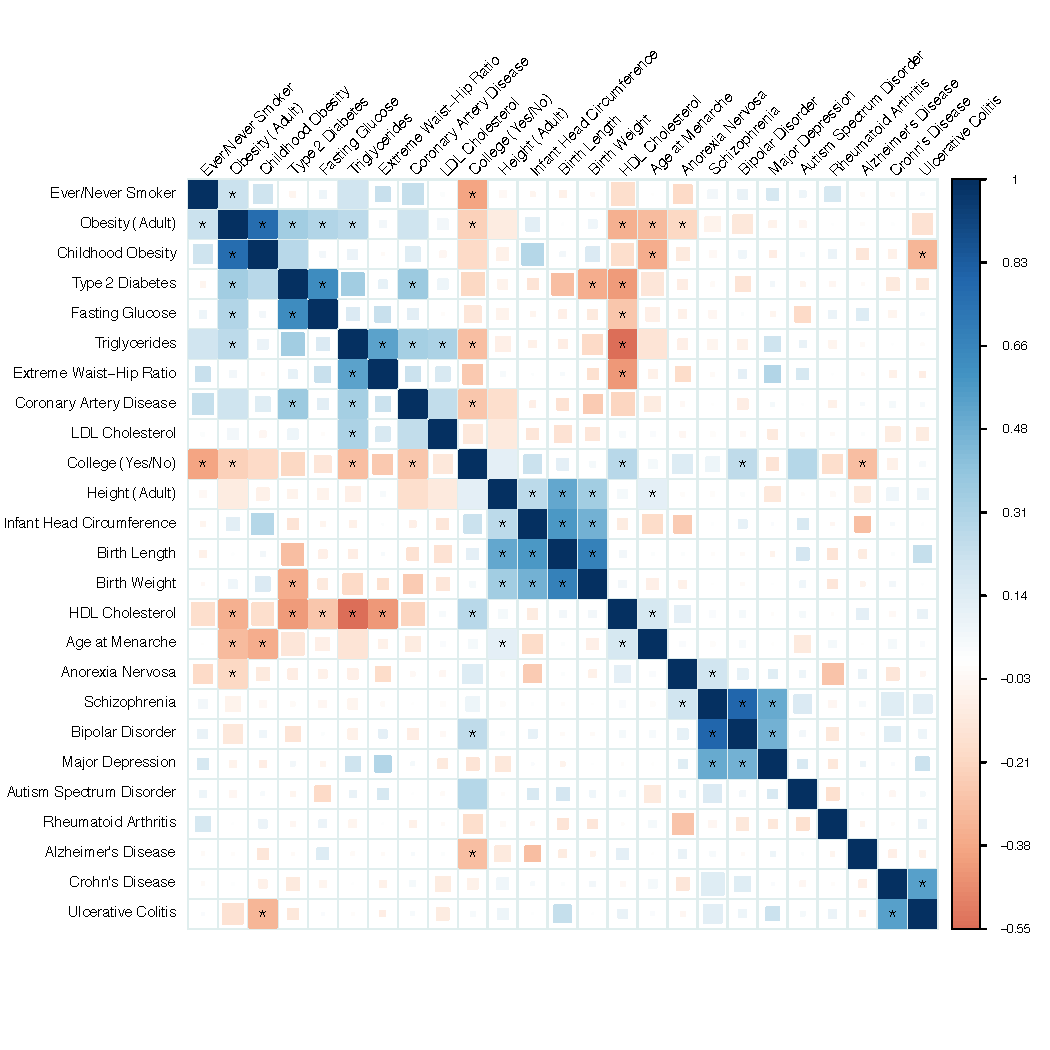
\includegraphics[scale=0.9]{figs/rg_heatmap.pdf}
         \label{Fig:300 Gencors}

Placeholder figure (HM3 LD Score). Caption goes here.
\end{centering}
\end{figure}
We find that phenotypes tend to cluster into categories defined by clinical practice and observational epidemiology;
for instance, we observe high genetic correlations between anthopometric traits, between psychiatric traits,  between 
metabolic traits and between autoimmune traits.
Reassuringly, most genetic correlations across categories were non-significantly different from zero.
%%% FACTOR ANALYSIS?

We observed some interesting individual results (Table \textbf{NNN}).
A few examples:
We estimate genetic correlations close to zero between Alzheimer's and all of the psychiatric traits.
Even though Alzheimer?s disease is classified as a psychiatric disorder in ICD-10, it appears to be genetically distinctive. 
Instead, Alzheimer's disease clusters (weakly, but significantly) with anthopometric traits.
We estimate genetic correlation close to zero between rheumatoid arthritis (RA) and schizophrenia, 
and between smoking traits and schizophrenia,
despite reduced risk of RA in patients with schizophrenia
and high rate of smoking in patients with schizophrenia

... etc more examples

%%%%%%%%%%%%%%%%%%%%%%%%%%%%%%%%%%%%%%%%%%%%%%%%%%%%%%%%%%%%%%%
\section{Discussion}\label{Discussion}
%%%%%%%%%%%%%%%%%%%%%%%%%%%%%%%%%%%%%%%%%%%%%%%%%%%%%%%%%%%%%%%\

\subsection{Limitations and Future Directions}
We note some limitations of LD Score regression. 
First, LD Score regression requires large sample sizes (at least a few thousand) in order to give estimates with reasonable
standard error. 
For smaller sample sizes, GCTA-REML is are more statistically efficient estimator of genetic correlation when its assumptions
are met (in particular, for non-ascertained studies) and individual genotypes are available.
In our opinion, figuring out how to obtain an efficient estimate of genetic correlation from a small and highly ascertained
sample (\emph{e.g.,} a study of a rare polygenic disease, where finding even a few thousand cases to genotype is challenging) 
is an open question.

Second, LD Score regression assumes that all individuals in the GWAS were sampled from populations with similar LD Scores,
and that these LD Scores can be estimated from sequence data.
For multi-continental GWAS, the solution is to run LD Score regression on each continental subcohort separately, 
but nevertheless, LD Score regression can only be applied to samples from populations for which there exists a large 
sequenced reference panel. 
Currently, LD Score regression cannot be applied to samples from admixed populations.
We provide a flowchart in Supplementary Figure \textbf{NNN} describing the situations in which LD Score regression is likely
to be useful for estimating genetic correlation.

Finally, while genetic correlations are less confounded than overall phenotypic correlations from observational
epidemiology, genetic correlations cannot be interpreted as causal effects, even genetic correlations between intermediate 
phenotypes and disease.
For example, consider the strong positive genetic correlation between LDL and CAD in Figure \ref{Fig:300 Gencors}.
This genetic correlation could result from a causal effect, \emph{e.g.,} $\mathrm{LD}\rightarrow\mathrm{CAD}$,
but could also result from shared genetic etiology 
\emph{e.g.,} $\mathrm{LDL}\leftarrow\mathrm{G}\rightarrow\mathrm{CAD}$, where $\mathrm{G}$ is some set of genetic factors.

Developing methods to distinguish between these models based on genetic data is a particularly exciting direction for future 
research.

\subsection{Data Sharing}

Under the header ``Minimum Viable Summary Statistics'' in the Methods.
\subsection{Recap}

\newpage
%%%%%%%%%%%%%%%%%%%%%%%%%%%%%%%%%%%%%%%%%%%%%%%%%%%%%%%%%%%%%%%
\section{Online Methods}\label{Online Methods}
%%%%%%%%%%%%%%%%%%%%%%%%%%%%%%%%%%%%%%%%%%%%%%%%%%%%%%%%%%%%%%%

%%%%%%%%%%%%%%%%%%%%%%%%%%%%%%%%%%%%%%%%%%%%%%%%%%%%%%%%%%%%%%%
\subsection{Statistical Framework}
%%%%%%%%%%%%%%%%%%%%%%%%%%%%%%%%%%%%%%%%%%%%%%%%%%%%%%%%%%%%%%%

See the supplementary note for a thorough derivation of the models behind LD Score regression.


%%%%%%%%%%%%%%%%%%%%%%%%%%%%%%%%%%%%%%%%%%%%%%%%%%%%%%%%%%%%%%%
\subsection{$h^2_{5\myhyphen50\%}$}
%%%%%%%%%%%%%%%%%%%%%%%%%%%%%%%%%%%%%%%%%%%%%%%%%%%%%%%%%%%%%%%

Let $S$ denote the set of all SNPs in 1000 Genomes (or whatever much larger sequenced reference panel future readers
are more familiar with); let $X_j$ denote the random variable whose value is the 0-1-2 coded genotype at SNP $j$, and let $y$
denote a phenotype. Let 
\begin{equation}
	\beta := \mathrm{argmax}_\alpha\left( \corr\left[y, \sum_{j\in S} X_j\alpha_j\right]^2 \right)
\end{equation}
(note that uniqueness of $\beta$ is guaranteed because this is a projection). 
Let $S'$ denote the set of SNPs with MAF$>5\%$. Then
\begin{equation}
	h^2_{5\myhyphen50\%} := \sum_{j\in S'} \beta_j^2.
\end{equation}
We choose 5\% as the lower bound, because we can estimate LD Scores for 5\% SNPs reasonably well from the $N=387$ 
samples in 1000 Genomes. With larger sample sizes in future sequenced reference panels, this lower bound can be pushed lower.

The main distinction between $h^2_{5\myhyphen50\%}$ and $h^2_g$ is that the effects of causal 4\% SNPs are not counted towards $h^2_{5\myhyphen50\%}$
This differs from the definition of the quantity $h^2_g$ estimated by GCTA-REML, in that GCTA-REML considers a set of SNPs
$g$, and then projects the phenotype onto those SNPs, without accounting for SNPs that are not in the set $g$. 
Thus if there is a 5\% SNP in set $g$ that is in high LD with a 4\% SNP that happens to be causal for the phenotype of interest
but is not in $g$, then the effect of the 4\% SNP is counted towards $h^2_g$ (or at least the component of the effect of 
the 4\% SNP that is tagged by the 5\% SNP that is in $g$).
There tends not to be very much LD between SNPs with different MAFs, 
so in the specific case of a MAF cutoff, this distinction likely makes only a small difference.

Technically, we should write $h^2_{5\myhyphen50\%,1kG}$ to indicate that we are only accounting for SNPs in 1000 Genomes,
but 1000 Genomes has sufficiently good power to observe 5\% and higher SNPs that we feel justified in omitting $1kG$
from the subscript for notational simplicity. 
It is perhaps more important to also note that we are only accounting for autosomal variation.
Most GWAS do not report summary statistics for SNPs on the sex chromosomes or in mitochondrial DNA.

Note that estimates of  $h^2_{5\myhyphen50\%}$ should generally be less than pedigree-based estimates of heritability
(modulo standard error), since pedigree estimators take into account all forms of genetic variation 
rare variants, microsatellites, indels, copy number variants, non-autosomal variation, etc).

The genetic covariance and genetic correlation quantitates that we estimate are direct bivariate analogues of 
$h^2_{5\myhyphen50\%}$. 
It is possible that the genetic covariance between two phenotype may be different among MAF$>5\%$ variants than
among rare variants; however, we could not detect such a phenomenon with GWAS data, since current GWAS only reliably
assay common variation.


%%%%%%%%%%%%%%%%%%%%%%%%%%%%%%%%%%%%%%%%%%%%%%%%%%%%%%%%%%%%%%%
\subsection{Estimation of LD Scores}
%%%%%%%%%%%%%%%%%%%%%%%%%%%%%%%%%%%%%%%%%%%%%%%%%%%%%%%%%%%%%%%

We estimated LD Scores from the European samples in the 1000 Genomes Project \cite{10002012integrated}
reference panel using the \texttt{--l2} flag in the \texttt{ldsc }software package by the authors (URLs) as in \cite{buliksullivan2014}.
We estimated per-allele LD Scores using the \texttt{--per-allele} flag in \texttt{ldsc}, and
we estimated MAF-binned LD Scores using the \texttt{--cts-bin} and \texttt{--cts-breaks} flags in \texttt{ldsc}.
Following \cite{buliksullivan2014}, we estimated LD Scores using a 1 centiMorgan (cM) window
(with the \texttt{ldsc} flag \texttt{--ld-wind-cm 1}).
Unlike \cite{buliksullivan2014}, we used a MAF cutoff of $1\%$ when estimating LD Scores,
in order to reduce the impact of LD measurement error on our regressions.
Since we only include variants with MAF $> 5\%$ in LD Score regressions for estimating genetic correlation,
and because there is very little LD between variants with MAF $> 5\%$ and variants with MAF $< 5\%$, 
this is unlikely to impact our results. 

For the analyses with HapMap 3 \cite{international2010integrating} LD Scores,
we took the sum of $r^2$'s over the same subset of HapMap 3 SNPs retained for LD Score regression in
\cite{buliksullivan2014}, (that is, HapMap 3 SNPs with MAF $> 1\%$, excluding centromeres and regions with long-range LD)
using the \texttt{--keep} flag in \texttt{ldsc}.


%%%%%%%%%%%%%%%%%%%%%%%%%%%%%%%%%%%%%%%%%%%%%%%%%%%%%%%%%%%%%%%
\subsection{Partitioned LD Score Regression}
%%%%%%%%%%%%%%%%%%%%%%%%%%%%%%%%%%%%%%%%%%%%%%%%%%%%%%%%%%%%%%%

In partitioned LD Score regression, we cut the set of SNPs in our reference panel into bins, for example,
we might use five MAF bins, corresponding to MAF 0-10\%, 10-20\%, ... , 40-50\% (as in supplementary table 4 of \cite{pgccdg2013}).  
We allow the variance explained per SNP to vary from bin to bin, but assume that variance explained per SNP is (roughly) 
equal within each bin. 
This amounts to approximating the unknown function that maps MAF to variance explained per SNP with a locally 
constant approximation. 
This presents a bias/variance tradeoff: if the mesh of our locally constant approximation is too coarse 
(\emph{e.g.,} if we were to use two MAF bins instead of five), 
our locally constant approximation would be poor, and this would result in bias. 
On the other hand, if we use too many bins, the standard error of our estimates will increase. 
However, we show in the simulations under the header ``Misspecified Models of Genetic Architecture" that
we can remove almost all MAF- and LD-bias under realistic parameter settings using only a few tens of bins, which 
increases the standard error only modestly.
MAF- and LD- partitioned LD Scores can be estimated using the \texttt{--cts-bin} and  \texttt{--cts-breaks} flags
from our \texttt{ldsc} software.


%%%%%%%%%%%%%%%%%%%%%%%%%%%%%%%%%%%%%%%%%%%%%%%%%%%%%%%%%%%%%%%
\subsection{Genetic Covariance Regression Weights} 
%%%%%%%%%%%%%%%%%%%%%%%%%%%%%%%%%%%%%%%%%%%%%%%%%%%%%%%%%%%%%%%

For heritability estimation, we use the LD Score regression weights derived in the 
supplementary note from \cite{buliksullivan2014}. 
The optimal regression weights for genetic covariance estimation are 
\begin{equation}
\var[\bhat_j\chat_j \,|\, \ell_j ] = 
	\left( 
		\frac{\hsqo\ell_j}{M} 
		+ 
		\frac{1-\hsqo}{N_1} 
	\right) \left(  
		\frac{\hsqt\ell_j}{M} 
		+ 
		\frac{1-\hsqt}{N_2}
	\right) 
	+ 					
	2\left( 
		\frac{\gencov\ell_j}{M} 
		+ 
		\frac{\rho N_s}{N_1N_2} 
	\right);
\end{equation}
(Supplementary Note) however, this quantity depends on both heritabilities, 
the genetic covariance and the number of overlapping samples,
which are often not known a priori, so some approximation is required.
In order to obtain approximate regression weights, 
we use heritability estimates from the single-phenotype LD Score regressions, then
we assume that $N_s$ is close enough to zero that the term $\rho N_s/N_1N_2$ is negligible
(though this default can be adjusted using the {-}{-}overlap and {-}{-}rho flags in \texttt{ldsc}),
and estimate a rough genetic covariance (which we only use for the regression weights)
using the aggregate estimator 
$$\hat{\rho}_{g, agg} := \frac{1}{\lbar\sqrt{N_1N_2}}\sum_{j=1}^M z_{1,j}z_{2,j},$$
where $\lbar$ denotes the mean LD Score among SNPs included in the regression.
These regression weights are only an approximation to the optimal weights,
but this will not introduce bias into the regression;
it will only increase the standard error. 
The standard errors for LD Score regressions with summary statistics 
from GWAS with sample size below 10,000 are low enough to be interpretable,
so non-optimality of the regression weights does not seem to be a major hindrance.

Users of our \texttt{ldsc} software package should note that when attempting to compute the genetic 
correlation between a trait and itself using the same GWAS data twice, the result will generally be different from 
one unless the weights are set appropriately. 
With the default weights (which are set for zero sample overlap), \texttt{ldsc} is simply computing the ratio
between the slope of and LD Score regression with efficient weights and the slope of an LD Score regression
with inefficient regression weights, which is equal to one in expectation, but with noise.

%%%%%%%%%%%%%%%%%%%%%%%%%%%%%%%%%%%%%%%%%%%%%%%%%%%%%%%%%%%%%%%
\subsection{Weighted Block Jackknife Genetic Correlation}
%%%%%%%%%%%%%%%%%%%%%%%%%%%%%%%%%%%%%%%%%%%%%%%%%%%%%%%%%%%%%%%

This section describes the implementation of the \texttt{--sumstats-gencor} flag in \texttt{ldsc}.

Genetic correlation is defined as a ratio of quantities: 
\begin{equation*}
	r_g := \frac{\gencov}{\sqrt{\hsqo\hsqt}}.
\end{equation*}
Instead of the naive estimator of this ratio, 
\begin{equation*}
	\rhat_{g} := \frac{\hat{\rho}_g }{ \sqrt{\hat{h}^2_1\hat{h}^2_2}},
\end{equation*}
we use the weighted block jackknife estimator \cite{busing1999delete} of the ratio, 
with the jackknife taken over blocks of adjacent SNPs
\begin{equation}
    \hat{r}_{g,jack} := 
    n_b\hat{r}_{g} -
     \sum_{i=1}^{n_b}
     	\left(1-\frac{m_i}{M_g}\right)\hat{r}_{g,i}
\end{equation}
where $n_b$ is the number of blocks, and $\hat{r}_{g,i}$ is
the naive estimate of genetic correlation obtained by deleting the $i^{th}$ block of SNPs, 
$m_i$ is the number of SNPs in block $i$, and $M_g$ is the number of SNPs included in the regression.
The weighted block jackknife ratio estimator is less biased than the naive estimate (though this is not so important at our sample sizes), 
and comes with a convenient nonparametric variance estimator \cite{busing1999delete},
\begin{equation}
    \widehat{\mathrm{Var}}\left[\hat{r}_{g,jack}\right] 
:= 
    \frac{1}{n_b} \sum_{i=1}^{n_b}
    	\frac{1}{h_i - 1}
	\left(
		(h_i-n_b)\hat{r}_g - (h_i-1)\hat{r}_{g,i} + \sum_{j=1}^{n_b} \left(1-\frac{m_i}{M_g}\hat{r}_{g,j}\right),
		\right)
\end{equation}
where $h_i := M_g / m_i$.
Weighted block jackknife standard errors (over blocks of adjacent SNPs) 
are robust to the  correlated error structure of GWAS $\chi^2$-statistics, 
so long as the block size exceeds the typical range of LD. 
See references \cite{buliksullivan2014, finucane2014partitioning, moorjani2011history} 
for examples of papers in the statistical and population genetics literature that use this technique. 
We checked the reliability of our standard errors via simulations with real genotypes
(Supplementary Table \ref{supp-se_sim}),
and found that the \texttt{ldsc} default setting  of 2000 blocks genome-wide
(which can be adjusted with the \texttt{--num-blocks} flag) gives standard error estimates
that agree well with the empirical standard deviation across simulation replicates.

In another set of simulations with much lower power (not shown), we observed that the LD Score regression
genetic correlation estimates became unstable when either sample size or heritability was so low that at least one 
of the two heritability estimates was not significantly different from zero. 
This is a general difficult with attempting to estimate a ratio where the denominator is close to zero, and is not 
specific to LD Score regression. 
As a rule of thumb, 
we recommend discarding (or at least being very cautious with) 
any genetic correlation estimates where either of the following conditions is met:
\begin{enumerate}
	\item Either of the heritability estimates is less than 2 SE's from zero, or
	\item The block jackknife SE for the genetic correlation estimate is greater than 0.2.
\end{enumerate}


%%%%%%%%%%%%%%%%%%%%%%%%%%%%%%%%%%%%%%%%%%%%%%%%%%%%%%%%%%%%%%%
\subsection{GWAS Data}
%%%%%%%%%%%%%%%%%%%%%%%%%%%%%%%%%%%%%%%%%%%%%%%%%%%%%%%%%%%%%%%

\subsubsection{Minimum Viable Summary Statistics}

The minimum summary data required for estimating genetic correlation with LD Score regression are the following:
\begin{enumerate}
	\item Genome-wide summary statistics from cohorts with similar ancestry
	\item The summary statistics must be \emph{signed} (allele and direction of effect)
	\item The summary statistics should \emph{never} be ``corrected'' via genomic control (GC) correction. Using GC'ed
		summary statistics will result in downward bias in the LD Score regression estimates of heritability and
		genetic covariance, and deflated LD Score regression intercepts, though the genetic correlation estimates will be fine.
	\item The summary statistics must not be meta-analyzed with targeted genotyping at significant loci 
		(\emph{e.g.,} specialty genotyping arrays like immunochip, exome chip, psychchip, metabochip, or replication cohorts) 
\end{enumerate}
The next details are nice to have, but are only used for filtering SNPs:
\begin{enumerate}
	\item A measure of imputation quality (\emph{e.g.,} INFO) for each SNP
	\item Sample size at each SNP (for binary traits, number of cases and number of controls)
	\item Sample MAF
\end{enumerate}
If these data are not available, 
we recommend retaining only HapMap 3 SNPs with reference panel MAF above 5\% for the LD Score regression as a workaround
(note: for \emph{regression}, not for estimation of the LD Scores), 
since HapMap3 SNPs seem to be well-imputed in most studies.


\subsubsection{Huge Effect Loci}

Though the derivation of LD Score regression makes no distributional assumptions about effect sizes, 
the LD Score regression standard error can become very large if effect sizes are drawn from a highly kurtotic distribution,
\emph{i.e.,} if there are huge-effect loci. 
The \texttt{ldsc} default is to remove a window around SNPs with $\chi^2 > 0.01N$
(this can be disabled with the \texttt{--no-filter-chisq} flag).


\subsubsection{IGAP}

IGAP (which provided the summary statistics for Alzheimer's disease) requests that we include the following text in our methods section:
\begin{quotation}
    International Genomics of Alzheimer's Project (IGAP) is a large two-stage study based upon genome-wide association studies (GWAS) on individuals of European ancestry. 
    In stage 1, IGAP used genotyped and imputed data on 7,055,881 single nucleotide polymorphisms (SNPs) to meta-analyze four previously-published GWAS datasets consisting of 17,008 Alzheimer's disease cases and 37,154 controls 
    (The European Alzheimer's disease Initiative, EADI; the Alzheimer Disease Genetics Consortium, ADGC; The Cohorts for Heart and Aging Research in Genomic Epidemiology consortium, CHARGE; The Genetic and Environmental Risk in AD consortium, GERAD). 
    In stage 2, 11,632 SNPs were genotyped and tested for association in an independent set of 8,572 Alzheimer's disease cases and 11,312 controls. 
    Finally, a meta-analysis was performed combining results from stages 1 and 2.
\end{quotation}
Note that we only used stage 1 data for LD Score regression.

\newpage
%%%%%%%%%%%%%%%%%%%%%%%%%%%%%%%%%%%%%%%%%%%%%%%%%%%%%%%%%%%%%%%
%\input{./tex/main/legends}
%%%%%%%%%%%%%%%%%%%%%%%%%%%%%%%%%%%%%%%%%%%%%%%%%%%%%%%%%%%%%%%


%%%%%%%%%%%%%%%%%%%%%%%%%%%%%%%%%%%%%%%%%%%%%%%%%%%%%%%%%%%%%%%
\section{URLs}\label{URLs}
%%%%%%%%%%%%%%%%%%%%%%%%%%%%%%%%%%%%%%%%%%%%%%%%%%%%%%%%%%%%%%%

\begin{enumerate}
	\item \texttt{ldsc} software:\\ 
		\texttt{github.com/bulik/ldsc}
		
	\item LD block genotype simulation code:\\
		\texttt{github.com/bulik/ldsc-sim}
		
	\item This paper:\\
		\texttt{github.com/bulik/gencor\_tex}
		
	\item PGC (psychiatric) summary statistics:\\ 
		\texttt{www.med.unc.edu/pgc/downloads}
		
	\item GIANT (anthopometric) summary statistics: \\
		\texttt{www.broadinstitute.org/collaboration/giant/index.php/GIANT\_consortium\_data\_files}
		
	\item MAGIC (insulin, glucose) summary statistics: \\
		\texttt{www.magicinvestigators.org/downloads/}
		
	\item CARDIoGRAM (coronary artery disease) summary statistics:\\	
		\texttt{www.cardiogramplusc4d.org}
	
	\item DIAGRAM (T2D) summary statistics:\\
		\texttt{www.diagram-consortium.org}
		
	\item Rheumatoid Arthritis summary statistics:\\
		\texttt{www.broadinstitute.org/ftp/pub/rheumatoid\_arthritis/Stahl\_etal\_2010NG/}
	
	\item IGAP (Alzheimers) summary statistics:\\
		\texttt{www.pasteur-lille.fr/en/recherche/u744/igap/igap\_download.php}

	\item IIBDGC (inflammatory bowel disease) summay statistics:\\
		\texttt{www.ibdgenetics.org/downloads.html}\\
		Note that we used a newer version of these data with 1000 Genomes imputation.

	\item Plasma Lipid summary statistics:\\
		\texttt{www.broadinstitute.org/mpg/pubs/lipids2010/}
	
	\item Beans:\\
		\texttt{www.barismo.com}\\
		\texttt{www.bluebottlecoffee.com}
\end{enumerate}

\newpage
%%%%%%%%%%%%%%%%%%%%%%%%%%%%%%%%%%%%%%%%%%%%%%%%%%%%%%%%%%%%%%%
\section{Acknowledgements}\label{Acknowledgements}
%%%%%%%%%%%%%%%%%%%%%%%%%%%%%%%%%%%%%%%%%%%%%%%%%%%%%%%%%%%%%%%

We would like to thank P. Sullivan and S. Caldwell for helpful discussion. This work was supported by NIH grants R01 HG006399 (ALP), R03 CA173785 (HKF) and by the Fannie and John Hertz Foundation (HKF). The coffee that Brendan drank while writing this paper was roasted by Barismo in Arlington, MA and Blue Bottle Coffee in Oakland, CA. 

Data on glycaemic traits have been contributed by MAGIC investigators and have been downloaded from www.magicinvestigators.org.

Data on coronary artery disease / myocardial infarction have been contributed by CARDIoGRAMplusC4D investigators and have been downloaded from 
www.CARDIOGRAMPLUSC4D.ORG

We thank the International Genomics of Alzheimer's Project (IGAP) for providing summary results data for these analyses. The investigators within IGAP contributed to the design and implementation of IGAP and/or provided data but did not participate in analysis or writing of this report. IGAP was made possible by the generous participation of the control subjects, the patients, and their families. The i-Select chips was funded by the French National Foundation on Alzheimer's disease and related disorders. EADI was supported by the LABEX (laboratory of excellence program investment for the future) DISTALZ grant, Inserm, Institut Pasteur de Lille, Universit� de Lille 2 and the Lille University Hospital. GERAD was supported by the Medical Research Council (Grant 503480), Alzheimer's Research UK (Grant 503176), the Wellcome Trust (Grant 082604/2/07/Z) and German Federal Ministry of Education and Research (BMBF): Competence Network Dementia (CND) grant 01GI0102, 01GI0711, 01GI0420. CHARGE was partly supported by the NIH/NIA grant R01 AG033193 and the NIA AG081220 and AGES contract N01-AG-12100, the NHLBI grant R01 HL105756, the Icelandic Heart Association, and the Erasmus Medical Center and Erasmus University. ADGC was supported by the NIH/NIA grants: U01 AG032984, U24 AG021886, U01 AG016976, and the Alzheimer's Association grant ADGC-10-196728.


%%%%%%%%%%%%%%%%%%%%%%%%%%%%%%%%%%%%%%%%%%%%%%%%%%%%%%%%%%%%%%%
\section{Author Contributions}\label{author_contribs}
%%%%%%%%%%%%%%%%%%%%%%%%%%%%%%%%%%%%%%%%%%%%%%%%%%%%%%%%%%%%%%%

The caffeine molecule is responsible for everything that is good about this manuscript.
BBS and HKF are probably responsible for the other bits.
All authors revised and approved the final manuscript.


%%%%%%%%%%%%%%%%%%%%%%%%%%%%%%%%%%%%%%%%%%%%%%%%%%%%%%%%%%%%%%%
\section{Competing Financial Interests}
%%%%%%%%%%%%%%%%%%%%%%%%%%%%%%%%%%%%%%%%%%%%%%%%%%%%%%%%%%%%%%%

Unfortunately, we have no financial conflicts of interest to declare.

\newpage
\bibliographystyle{plain}
\bibliography{gencor}

\end{document}
